%% Overlapping construction plus a position-blind split.
%% OUP Bioinformatics Advances (Modern, Large), author-year. Resubmission of BIOADV-2026-296,
%% restructured to the construction-defect-first spine. (This file was briefly named main_8pp.tex,
%% for an 8-page Original Article budget that turned out not to apply; the name is gone with it.)
%% Numeric conventions: .predict()/argmax decision rule; 5-seed-mean corrected accuracy;
%% test-set percentile bootstrap or cluster (block) bootstrap 95% CI as stated per number.
%% tab_reportcard.tex is GENERATED by audit.pipeline.emit_tables -- never edit it by hand; edit the
%% source CSV and rebuild. tab_roster.tex is likewise generated and is \input by supplementary.tex.
\documentclass[webpdf,modern,large,namedate]{oup-authoring-template}%

\graphicspath{{Fig/}}
\emergencystretch=1.5em

\begin{document}

\journaltitle{Bioinformatics Advances}
\DOI{DOI added during production}% pre-acceptance stub, verbatim from oup-authoring-template
\copyrightyear{2026}% confirm at acceptance
\pubyear{2026}% confirm at acceptance
\vol{XX}% pre-acceptance stub; fills the running head
\issue{X}% pre-acceptance stub; fills the running head
\volume{Volume XX, Issue X}% distinct class hook from \vol/\issue; fills the page-1 citation line
\access{Published: Date added during production}% pre-acceptance stub
\appnotes{Original Article}

\firstpage{1}% pre-acceptance stub

\title[Overlapping construction and a position-blind split]{Overlapping construction plus a position-blind split: a curation defect in genomic sequence benchmarks and the model rankings it inverts}

%% ===== Author / affiliation =====
\author[1,$\ast$]{Rikhin Kavuru}
\address[1]{\orgname{Independent Researcher}, \country{United States}}
\corresp[$\ast$]{Corresponding author. \href{mailto:rikhinkavuru@gmail.com}{rikhinkavuru@gmail.com}}

\abstract{
\textbf{Motivation:} Genomic benchmarks rarely control for near-duplicate sequences spanning their train/test split. A model can then score by recognizing memorized near-copies rather than generalizing, and no audit locates its origin.\\
\textbf{Results:} Near-duplicate leakage here requires two conditions together---an overlapping construction step and a split that ignores genomic position---rather than any property of the sequence type. A pre-registered prediction that short human regulatory tasks would be leaky failed: those GUE tasks are clean at full scale across seven independent partitions (eleven shipped tasks). The signature precedes any model: in Genomic Benchmarks the leaky positive class ships $77{,}421$ intervals on $40{,}934$ distinct coordinates, and a coordinate screen whose verdict cut is inherited rather than fitted separates seven of eight datasets. The defect is causal both ways: the omitted merge step drops the leak fraction from $0.390$ to $0.012$ and the random forest's gap from $+0.165$ to $-0.008$; imposing duplication manufactures both in a clean dataset. The headline drop separates into two effects that a single number hides: on \textit{human\_enhancers\_ensembl} $9.0$ of the memorizing forest's $16.4$ points is \emph{evaluation-side} inflation, measurable on the novel stratum with no retraining and no re-split, and the remaining $7.4$ is a retraining penalty paid by that model alone. The shipped split then materially distorts model comparison, and can invert it: it leaves the top three of nine learners within $0.0015$, yet corrected they span $23$ points---more than a difficulty-matched test set at the same accuracy produces ($14$), and on two clean datasets the same re-split expands spread not at all; a from-scratch CNN ranks fifth of ten as shipped and first corrected. The inversion is conditional, and we state its conditions rather than generalize past them: it requires a memorization-prone learner in the comparison set, and imposing the same construction defect on three independent clean datasets manufactures the inflation in all three and the reordering in two, the exception being a donor whose memorizer already ranked last. Among shipped datasets it is an existence proof on one: \textit{human\_nontata\_promoters} certifies \emph{leaky-but-correction-unsafe}, its demotion does not survive AUROC or $F_1$, and it is reported as a negative rather than as a second demonstration.\\
\textbf{Availability and implementation:} Code, the report card, a near-duplicate-aware splitter and a certification tool are at \url{https://github.com/rikhinkavuru/homology-leakage-genomic-benchmarks}.\\
\textbf{Contact:} \href{mailto:rikhinkavuru@gmail.com}{rikhinkavuru@gmail.com}\\
\textbf{Supplementary information:} Available at \textit{Bioinformatics Advances} online.}

\keywords{data leakage, near-duplicate sequences, benchmark evaluation, genomics, model ranking}

\maketitle

\section{Introduction}\label{sec:intro}

Benchmark suites are the default proving grounds for new DNA sequence classification methods, and the Genomic Benchmarks collection \citep{gresova2023} is used in part because it is small and quick to run. The value of any such suite rests critically on one assumption among several: that its train/test split measures generalization rather than recall of the training data. Near-duplicate leakage---exact or near-identical sequences appearing on both sides of a split---breaks that assumption, because a model can then succeed by recognizing memorized near-copies, so reported accuracy overstates generalization.

The evidence for such leakage can sit in files distributed with the benchmark, before any model is trained. The positive class of \textit{human\_enhancers\_ensembl} ships $77{,}421$ genomic intervals on only $40{,}934$ distinct coordinates: $36{,}487$ coordinates appear exactly twice and $4{,}447$ once, so $94.3\%$ of positive rows sit on a duplicated coordinate, and because the shipped split is random, $75.5\%$ of test positives have their exact coordinate present in training. A near-default random forest ($150$ trees, \texttt{min\_samples\_leaf=1}) scores $0.860$ on that split and $0.696$ once the near-copies are removed; on the near-duplicate test sequences alone it scores $1.000$, and on the rest $0.770$---worse than the linear SVM it outranks. Four of the suite's seven binary datasets carry none of this, one is borderline under a length-robust metric, and two are leaky, so the defect is a property of particular datasets rather than of the suite.

Leakage is an established benchmarking hazard. \citet{kapoor2023leakage} document it as a pervasive driver of the reproducibility crisis in ML-based science, inflating performance and, in extreme cases, changing the apparent ordering of methods. In genomics, hashFrag \citep{rafi2026} shows homologous sequences spanning cis-regulatory splits inflating neural-model performance, and reports that models rely on memorized associations wherever function is conserved between homologs; standard protein-interaction splits leave most test cases with near-duplicate counterparts \citep{bushuiev2024}; de-leaked test sets sharply reduce reported performance including for AlphaFold-Multimer \citep{kovtun2024}; and on LIT-PCBA a trivial memorization baseline matches sophisticated methods because the benchmark is leaky \citep{huang2025}. Evaluation design is itself a recognized genomics hazard \citep{whalen2022pitfalls,schreiber2020pitfall,toneyan2022evaluating}. Outside biology the ranking question has been posed most sharply: \citet{barz2020cifar} find near-duplicates of training images inside the CIFAR test sets, \citet{northcutt2021labelerrors} show test-set defects destabilizing the ranking of models evaluated on ten widely used benchmarks, and under controlled injection \citet{zhou2023cheater} show benchmark leakage distorting model comparison, a hazard established at scale by work on train/test overlap, corpus deduplication and language-model contamination \citep{elangovan2021leakage,lee2022dedup,sainz2023contamination,magar2022contamination,deng2024contamination}. The usual remedy is a similarity-aware partition \citep{hobohm1992,walsh2016correct,teufel2023graphpart,petti2022benchmark,li2006cdhit,steinegger2017mmseqs2}.

None of that is in dispute, and none of it is what this paper claims to have discovered. Leakage, near-duplicate contamination and similarity-aware partitioning are established topics, and in genomics specifically hashFrag \citep{rafi2026} has already shown homologous sequences spanning cis-regulatory splits inflating neural-model performance. Our contribution is narrower than the problem and is stated as such. First, the leakage in this suite is traced to a specific, documented, editable step in how the data were assembled---an omitted merge---rather than described as a property of the sequences. Second, it is detectable in the coordinate annotations shipped with the benchmark, before any model is trained, by a screen that needs no aligner, no sequence comparison and no fitted parameter. Third, that step is intervened on in both directions---removed from a leaky dataset, imposed on clean ones---so the link between construction and consequence is causal rather than correlational. Fourth, the consequence measured is a change in \emph{which model wins}, not only in how well models score. A fifth is a negative result: a prediction committed before the target suite was examined, that leakage would track task type, failed on every task it named. What that literature lacks, and a small curated suite supplies, is a matched clean control inside the same collection and a construction step that can be edited. The open question is accordingly upstream of the remedy: not how to repair a leaky split, but where the leakage originates and whether it reorders which model wins. Two candidate answers are separable. Leakage may track what a dataset contains---sequence type, task, window length---in which case a practitioner can screen by task family. Or it may track how the dataset was assembled, in which case the screen belongs in coordinate space and the fix belongs in the curation pipeline. Distinguishing them requires a prediction committed in advance and an intervention on the construction step alone. Pretrained foundation models are outside this evidence: DNABERT-2 \citep{zhou2023dnabert2}, HyenaDNA \citep{nguyen2023hyenadna} and the Nucleotide Transformer \citep{dallatorre2024nucleotide} all pretrain on the GRCh38 human reference---HyenaDNA on it alone, the other two as the human component of a multispecies corpus---and these test sequences lie in it (\S\ref{sec:d-pretrain}), so evaluating them would open a second, pretraining-based leakage channel no split can close.

Across the datasets audited here, leakage tracks how a dataset was assembled rather than what kind of sequence it contains, and the condition it requires is conjunctive: an overlapping construction step \emph{and} a split that ignores genomic position (\S\ref{sec:discussion}). Where similarity is instead a property of the sequences themselves---GUE's \textit{virus\_covid}, whose nine SARS-CoV-2 variants differ by a handful of mutations---a leak fraction of $1.000$ is biology and carries no information about curation (\S\ref{sec:d-detector}). We measure a coordinate-space signature on the shipped genomic intervals rather than the sequences, and a screen whose verdict cut is inherited rather than fitted separates the suite $7/8$ and calls four out-of-suite BEND partitions clean; we edit the construction step in both directions, applying the omitted merge step to a leaky dataset to abolish the leakage and its downstream consequences, and imposing it on a clean dataset to manufacture both; and we score a prediction committed before the target suite was examined, that GUE's short human regulatory tasks would be leaky, which failed---all eleven are clean at full scale, refuting the task-type hypothesis the prediction encoded. The downstream cost is that the shipped split materially distorts model comparison and can invert it, demonstrated on \textit{human\_enhancers\_ensembl}, where the as-shipped split does not separate its top three of nine learners---within $0.0015$---yet those three span $23$ accuracy points corrected, more than the $14$ a difficulty-matched test set at the same operating point produces. That demonstration is conditional, and the conditions are measured rather than assumed. It requires a memorization-prone learner in the comparison set and a challenger genuinely better on novel sequences; given both, the reordering appears on one shipped dataset, is manufactured on demand on two of three independent clean donors under intervention, and is absent from a second suite that supplies leakage without such a challenger. Both shipped datasets carrying the leakage are short human regulatory sets, one fixed at $251$\,bp and one variable at a $269$\,bp median over a $2$--$573$ range, so that regime remains a possible further necessary condition, and is not a sufficient one. We release a per-dataset report card, an aligner-free near-duplicate-aware splitter, and a certification tool returning \emph{leaky-but-correction-unsafe} where whole-cluster correction is not safe.

\section{Methods}\label{sec:methods}

\subsection{Datasets}\label{sec:m-data}
We study the seven binary Genomic Benchmarks datasets \citep{gresova2023} and additionally report the three-class \textit{human\_ensembl\_regulatory} set; sizes, lengths and balance are in Supplementary Table~S1. Their upstream provenance is pinned rather than assumed: per the curators' own construction notebooks, \textit{human\_nontata\_promoters} and \textit{human\_enhancers\_cohn} derive from the Ensembl release-$97$ GRCh38 toplevel DNA FASTA, and \textit{human\_enhancers\_ensembl} and \textit{human\_ocr\_ensembl} from the release-$100$ Regulatory Build external-feature table over the release-$100$ GRCh38 primary assembly. Every upstream URL was re-resolved on 2026-07-20 (all HTTP $200$; \texttt{results/reference\_provenance.csv}), and archive hosts are recorded alongside the live ones---\url{https://jul2019.archive.ensembl.org} for release $97$ and \url{https://apr2020.archive.ensembl.org} for release $100$---because Ensembl release $116$ (June 2026) is the last served on the current platform, with data moving to a new site from summer 2026, so the live paths in the notebooks are not durable citations. Balanced datasets are curated to $0.500$ positive fraction in both train and test, so class balance is preprocessed, not natural. All censuses and leak fractions are full-scale; four accuracy deltas are not. The corrected-split deltas for \textit{human\_ocr\_ensembl}, \textit{demo\_human\_or\_worm} and \textit{human\_enhancers\_cohn}, and the clean-control roster arm of \S\ref{sec:r-rank}, run on $20{,}000$-sequence subsamples of datasets whose report-card column is headed $n$ (full). Their full-scale leak fractions are $\le0.012$ (Jaccard) and $\le0.068$ (containment) for the three binary sets, and subsampling can only \emph{hide} leakage, so a subsample is admissible there to confirm cleanliness---never to establish it. The three-class set is bounded on the Jaccard side alone ($0.005$ at full scale): its full-scale containment was never computed, and since containment is precisely what moved \textit{demo\_coding\_vs\_intergenomic\_seqs} from clean to borderline in Table~\ref{tab:reportcard}, we state that gap rather than let the binary sets' bound stand in for it. On a $20{,}000$-sequence subsample its containment reads $0.014$, which by the same one-way argument confirms nothing.

\subsection{Coordinate-space construction signatures}\label{sec:m-coord}
Genomic Benchmarks distributes per-sequence intervals (\texttt{id,region,start,end,strand}) separately from the sequences its loader returns. We recover them offline and realign them to loader row order, which is deterministic (split, then sorted class directory, then sorted filename, the stem being the interval \texttt{id}); recovered interval width equals sequence length for $100\%$ of rows in all eight datasets, a check informative only for the four variable-length ones. These coordinates are read on a separate code path from the $k$-mer clustering and are causally upstream of it, so they give non-circular corroboration rather than a restatement. Per class we compute self-overlap redundancy $R_{\mathrm{self}}=1-n_{\mathrm{merged}}/n_{\mathrm{raw}}$ and the share of \emph{test} intervals overlapping any \emph{train} interval at $\ge t$ reciprocal overlap, $t\in\{{\ge}1\,\mathrm{bp},0.5,0.9,1.0\}$; overlap is strand-agnostic, strand being unrecorded for the two \textit{demo} datasets. The screen thresholds the maximum over classes of the $\ge50\%$ statistic at $0.1$. The $0.1$ verdict cut is carried over unchanged from sequence space and so adds no fitted parameter; the $\ge50\%$ overlap criterion is a second choice, made from the same $t\in\{{\ge}1\,\mathrm{bp},0.5,0.9,1.0\}$ grid on these eight datasets, because mere adjacency over-calls tiled data---\textit{drosophila\_enhancers\_stark} tiles at a $2{,}142$\,bp median and reads $0.406$ at ${\ge}1$\,bp against $0.036$ at $\ge50\%$. That criterion is therefore selected, not inherited, and the screen is parameter-free only in its verdict cut.

The assembly is measured, not assumed, and the unsampled check is the stronger one. All $190{,}973$ shipped intervals of the two leaky datasets name a primary chromosome and none an alternate contig, and---without sampling, so with no denominator to choose---$915$ of them ($0.48\%$) end past a GRCh37 chromosome boundary while none ends past a GRCh38 one. A sampled sequence-level check agrees. For $49$ test intervals stratified over both datasets, classes and strands we fetched the reference at the shipped coordinates from GRCh38 and GRCh37 via the UCSC REST API on 2026-07-20---\texttt{hg38}, the Dec.\ 2013 assembly, accession GCA\_000001405.15, and \texttt{hg19}, the Feb.\ 2009 assembly, accession GCA\_000001405.1---reading intervals as $0$-based half-open and reverse-complementing minus-strand records: GRCh38 reproduces the shipped sequence in $49$ of $49$ cases and a $1$-based reading in none of $49$. The GRCh37 denominator is $48$, not $49$, for the same reason the boundary count gives: one sampled chrX interval runs past the GRCh37 chromosome end, so the API returns an error rather than a sequence and that row is unevaluable on GRCh37 by construction. On the $48$ evaluable rows GRCh37 reproduces the shipped sequence once.

\subsection{Construct-and-break manipulations}\label{sec:m-manip}
We intervene on the construction step alone. \emph{Fix-a-leaky}: \textit{human\_enhancers\_ensembl} receives the merge step its curators omitted---every duplicated coordinate collapsed to one representative row---with sequences, labels, model code and split ratio unchanged and negatives subsampled to restore the control's balance. \emph{Break-a-clean}: \textit{human\_ocr\_ensembl}, drawn from the merged Ensembl Regulatory Build and clean by every measure, is rebuilt as an un-deduplicated assembly, duplicating positives until the same $94.3\%$ share of positive rows sits on a multiplicity-$2$ coordinate as on \textit{human\_enhancers\_ensembl} (requiring $89.1\%$ of them, since duplicating a fraction $r$ leaves $2r/(1+r)$ of rows on a duplicated coordinate), then downsampling to the control's exact size and class balance. Each manipulation is paired with an unmanipulated control at the same split seed. In both manipulated datasets the duplicated coordinates sit in the positive class, so both interventions perturb balance and size unless corrected; balance-matched arms are primary, and the break-a-clean pair is matched on size as well while the fix-a-leaky pair cannot be, since size there cannot be equalised without discarding the rows the intervention is defined to remove. A ten-dose version sweeps the imposed duplication rate (Supplementary \S S2).

\subsection{Near-duplicate measurement and re-split}\label{sec:m-measure}
We measure train/test overlap by the exact Jaccard similarity of $k$-mer sets ($k=8$) over all test--train pairs via sparse binary matrix products; the leakage fraction is the share of test sequences whose maximum similarity to any training sequence exceeds a threshold ($0.5$, $0.7$, $0.9$). A $k$-mer Jaccard is bounded by the length ratio, so it undercounts leakage on datasets with disparate lengths---across \textit{human\_enhancers\_ensembl}'s test--train pairs, $61\%$ have their Jaccard held below $0.7$ by length ratio alone---so we also report the length-robust \emph{containment} index $|A\cap B|/\min(|A|,|B|)$. Jaccard leak fractions are lower bounds; unfloored containment runs the other way and is an \emph{upper} bound on variable-length data, since a very short sequence is contained in almost anything. Calibrated on synthetic sequences with known ground truth, the $8$-mer Jaccard at $0.7$ detects an exact copy, one point mutation and a window shifted by up to $10\%$ of its length at every length we use, but at $70$\,bp it misses two point mutations $70\%$ of the time where at $\ge300$\,bp it tolerates five: a near-exact-duplicate detector on short sequences, a homology detector on long ones, so threshold choice should follow length (Supplementary \S S4). We separately census exact byte-identical duplicates on a code path using no $k$-mers: \textit{human\_enhancers\_ensembl} has $11{,}774$ such test sequences ($0.380$ of its test set), whereas \textit{human\_nontata\_promoters} has $0$ exact duplicates yet $0.225$ near-duplicates at Jaccard $\ge0.9$---the more homology-like but statistically weaker case.

To correct leakage we connect sequences whose Jaccard exceeds $0.7$, take connected components as clusters, and assign whole clusters to train or test, preserving the original ratio and balance and guaranteeing zero residual cross-split similarity above the threshold. Sweeping the threshold, the drop is flat on \textit{human\_enhancers\_ensembl} ($0.156/0.156/0.157$ at $0.5/0.7/0.9$; $0.158$ under largest-component removal) but scales strongly on \textit{human\_nontata\_promoters} ($0.205/0.121/0.006$), since $0.9$ leaves its large $[0.5,0.9)$ band uncorrected. This is an aligner-free instance of GraphPart's whole-cluster partitioning \citep{teufel2023graphpart}; an MMseqs2 arm is in Supplementary \S S3.

\subsection{Models, decision rule and pre-registration}\label{sec:m-models}
Sequences are represented by overlapping $k$-mer counts, $k\in\{4,6\}$. Nine classifiers span \emph{memorization propensity} (equivalently, effective regularization) rather than raw capacity: logistic regression, a linear SVM (\texttt{LinearSVC}), a random forest ($150$ trees at scikit-learn defaults, \texttt{min\_samples\_leaf=1}), \texttt{HistGradientBoosting}, extremely randomized trees, $1$- and $15$-nearest neighbours, a multilayer perceptron (MLP) and Gaussian naive Bayes; the first four constitute the four-model comparison, all nine the roster. Scale-sensitive learners receive L2 normalization, tree ensembles raw counts. All are trained from scratch on each split, so none carries a pretraining confound. Accuracies use \texttt{.predict()} (\texttt{argmax}); the headline drop is the original accuracy minus the mean corrected accuracy over five re-split seeds. Parameters and roster rationale: Supplementary \S S1. An inversion criterion built for four models is too permissive for nine---``the top model changed by more than a point'' fires on a \emph{clean} control from repartitioning alone---so we additionally require that the two models exchanging the top slot each lead on their own split by a \emph{paired} cluster-bootstrap difference excluding zero, and we report the swap margin separately from the as-shipped first-to-second margin, which can be a tie when the former is large.

The deep-model probe is a from-scratch 1D residual convolutional network in the Basset \citep{kelley2016basset} / DeepSEA \citep{zhou2015deepsea} lineage (one-hot input, no $k$-mer features), trained on each dataset's training split only. We pre-specified, in a document committed alongside the results it predicts, the narrowed claim, a dropout$\times$weight-decay grid, and a refutation condition: if the standard-practice regularized cell (dropout $0.3$, weight decay $10^{-4}$) has a cluster-bootstrap drop CI including $0$ on \emph{both} datasets, the strong ``any expressive learner is inflated'' reading is refuted and reported as a limitation. This is a binding stated condition, not an externally timestamped registration; it was committed in the same commit as the experiment code and so carries no priority evidence at all, unlike the cross-suite registration below. Commit hashes and timestamps for both, with the \texttt{git log} output that establishes the ordering and an explicit statement of what author-controlled timestamps can and cannot show, are published as \texttt{PREREGISTRATION.md} in the code repository.

Six predictions, P1--P6, were committed in code inside the module that would test each,
before that module was run, and all six are scored in the Results whether or not they held; they are
enumerated verbatim in Supplementary \S S1.9. Separately, before that suite was examined, we
registered for GUE \citep{zhou2023dnabert2} that its short fixed-length human regulatory tasks would
be leaky and its multi-species tasks clean (\S\ref{sec:r-gue}).

The \emph{graded memorization gap} is $\mathrm{acc}[\ge0.9]-\mathrm{acc}[<0.5]$. Raw, it is confounded: the strata differ sharply in class composition, in opposite directions on the two leaky datasets, and a constant classifier that memorizes nothing scores $+0.803$ on \textit{human\_enhancers\_ensembl} and $-0.980$ on \textit{human\_nontata\_promoters}. We therefore report the gap from \emph{balanced} accuracy within each stratum, for which a constant classifier scores exactly zero, alongside the raw gap so the confound stays visible (Supplementary \S S1).

\subsection{Controls, cross-suite census and intervals}\label{sec:m-controls}
\paragraph{Chromosome holdout and regularization.} Using the recovered coordinates we assign whole chromosomes to the test side in a single greedy pass until the target test fraction is reached (nine chromosomes for \textit{human\_enhancers\_ensembl}, twelve for \textit{human\_nontata\_promoters}; there is no cross-validation loop). This field-standard control is deployment-relevant but \emph{not} leakage-free: residual leakage at Jaccard $0.7$ is $0.8\%$ and $0.02\%$, against the exact $0$ the near-duplicate-aware split guarantees. Separately we sweep, for the random forest only, \texttt{min\_samples\_leaf}$\in\{1,5,20,50,100,200,500\}$ and \texttt{max\_depth}$\in\{\text{None},16,8,4\}$ at full scale---the largest settings exceed the largest cluster, so no leaf can be a pure duplicate block---and cross-validate the same leaf grid on the as-shipped \emph{training} set under ordinary stratified and cluster-grouped $5$-fold.

\paragraph{Cross-suite census.} The census is applied unchanged to the Nucleotide Transformer downstream tasks \citep{dallatorre2024nucleotide} and to GUE \citep{zhou2023dnabert2}; the full pipeline is then run on the tasks the first flags, with a clean task as control. Collapsing two nestings leaves eleven independent tasks of the thirteen shipped, and we report independent-task counts throughout; the three splice tasks are not nested and count separately, and we draw no before-and-after inference between the original and revised releases, which are not the same data recurated. One deviation affects the anchoring task: \textit{enhancers} ships only $400$ test sequences, too few for a usable interval, so for that task alone we pool train and test and draw a fresh stratified $80/20$ split before running both arms. Pooling redistributes the duplicate pairs, so the re-split leak fraction ($\varphi=0.099$) is not the same quantity as the $25\%$ byte-identical figure the as-shipped split carries (Supplementary \S S1).

\paragraph{Injected multiclass construction.} The only multiclass set is clean, so we answer the question by construction, injecting label-carrying near-duplicate train$\to$test copies. Here $f$ is the fraction of \emph{training} rows copied and appended to the test set, so realised test-set leak fractions are $\varphi=0.29$, $0.44$ and $0.62$ at $f=0.1$, $0.2$, $0.4$, not $f$. The arm runs on a $20{,}000$-sequence subsample; the dose is imposed rather than measured, so scale is not load-bearing.

\paragraph{Intervals and reproducibility.} Because near-duplicates violate the
independence a sample-wise bootstrap assumes, every interval resamples whole within-test
near-duplicate components as blocks on \emph{both} arms, and design effects, the cluster-versus-sample
variance ratio, a cluster-robust cross-check and a combined-source interval folding re-split-seed
variance are reported alongside. Percentile bootstrap draw counts are not uniform---$10{,}000$ for the headline drop and
threshold arms, $1{,}000$ for the manipulation, roster and cross-suite arms---and are stated
per arm in Supplementary \S S1.9. Benjamini--Hochberg at $q=0.05$ is applied over a declared
family of $15$ deltas \citep{benjamini1995fdr}. Models are not refit while the test set is resampled, so every
interval is conditional on the fitted models. Full definitions, the family membership rule, the
$p$-value approximation and the software environment are in Supplementary \S S1.9--S1.10.

\section{Results}\label{sec:results}

\subsection{Which datasets are leaky, and why the metric matters}\label{sec:r-card}
Only \textit{human\_enhancers\_ensembl} and \textit{human\_nontata\_promoters} exceed a $10\%$ near-duplicate test fraction at Jaccard $0.7$ ($0.384$, $0.406$); the three-class set is clean at $0.005$ (Table~\ref{tab:reportcard}). Re-measuring at full scale with containment reveals substantially more leakage on \textit{human\_enhancers\_ensembl} ($0.384\to0.845$) and flags one dataset the length-blind metric misses: \textit{demo\_coding\_vs\_intergenomic\_seqs}, clean under Jaccard ($0.078$), crosses the cut under containment ($0.131$), so we relabel it \emph{borderline}. The remaining four stay well below under both metrics (largest containment $0.068$). Two datasets are leaky---one of them, \textit{human\_nontata\_promoters}, certified \emph{leaky-but-correction-unsafe} because its largest-cluster cohesion is $0.083$, so whole-cluster correction would strip genuine signal along with the leakage---one borderline, four clean. A clean verdict moved, so both metrics should be reported.

\begin{table*}[tbp]
\begin{center}
\begin{minipage}{\textwidth}
\caption{Near-duplicate leakage report card. \textbf{Verdict} is LEAKY if the full-scale near-duplicate test fraction exceeds $0.1$ at Jaccard $0.7$; a ``clean'' verdict means only \emph{no forward-strand near-duplicate leakage detected}, subject to the disclosed length-pair cap---it is not a certificate of homology-freedom. ``leak@0.7 (Jac / con)'' gives the leak fraction under the $8$-mer Jaccard and the length-robust containment index; ``Acc.\ lost'' is the best-model accuracy change under the near-duplicate-aware re-split (positive $=$ accuracy lost). Leak fractions and censuses are full-scale on every row, but four of these deltas---\textit{human\_ocr\_ensembl}, \textit{demo\_human\_or\_worm}, \textit{human\_enhancers\_cohn} and the three-class \textit{human\_ensembl\_regulatory}---are computed on $20{,}000$-sequence subsamples of the datasets whose $n$ column is headed \emph{full}. Subsampling can only hide leakage, never create it, so a subsampled delta is admissible here to \emph{confirm} cleanliness and never to establish it (\S\ref{sec:m-data}). \textit{demo\_coding\_vs\_intergenomic\_seqs} is \emph{not} in that group: its delta is full-scale at $n=100{,}000$. $^{\dagger}$\textit{demo\_coding\_vs\_intergenomic\_seqs} is clean under Jaccard but borderline under containment. $^{\ddagger}$\emph{leaky-but-correction-unsafe}: the verdict the certification tool returns for a LEAKY dataset whose largest-cluster cohesion falls below $0.5$ (\textit{human\_nontata\_promoters}, $0.083$). Its near-duplicate components are single-linkage chains rather than sets of mutual near-copies, so whole-cluster re-splitting quarantines related but non-duplicate sequences and removes genuine signal along with the leakage. The leakage verdict stands; it is the \emph{corrected} delta on that row that cannot be read as a clean measurement, and the novel-stratum accuracy on the as-shipped split should be reported in its place.\label{tab:reportcard}}
\resizebox{\textwidth}{!}{% GENERATED by audit/pipeline/emit_tables.py -- do not edit by hand.
% Edit the source CSV and re-run, or the next build will overwrite you.
\begin{tabular}{@{}lrrrlrll@{}}
\toprule
Dataset & $n$ (full) & leak@0.7 (Jac) & leak@0.7 (con) & Verdict & Acc.\ lost & RF rank & Reorders under chrom.-holdout?\\
\midrule
human\_nontata\_promoters & 36{,}131 & 0.406 & 0.445 & \textbf{LEAKY} & $+0.118$ & $1\!\to\!3$ & no (RF stays rank~1)\\
human\_enhancers\_ensembl & 154{,}842 & 0.384 & 0.845 & \textbf{LEAKY} & $+0.165$ & $1\!\to\!4$ & yes (RF $\to$ rank~4)\\
demo\_coding\_vs\_intergenomic\_seqs & 100{,}000 & 0.078 & \textbf{0.131} & borderline$^{\dagger}$ & $-0.001$ & $4\!\to\!4$ & n/a\\
human\_ocr\_ensembl & 174{,}756 & 0.010 & 0.068 & clean & $+0.004$ & $4\!\to\!4$ & n/a\\
demo\_human\_or\_worm & 100{,}000 & 0.012 & 0.042 & clean & $-0.004$ & $4\!\to\!4$ & n/a\\
drosophila\_enhancers\_stark & 6{,}914 & 0.016 & 0.033 & clean & $+0.012$ & $2\!\to\!3$ & n/a\\
human\_enhancers\_cohn & 27{,}791 & 0.001 & 0.005 & clean & $-0.004$ & $4\!\to\!4$ & n/a\\
\midrule
human\_ensembl\_regulatory (3-class) & 289{,}061 & 0.005 & -- & clean & $-0.010$ & n/a & n/a\\
\botrule
\end{tabular}
}
\end{minipage}
\end{center}
\end{table*}

\subsection{The cause: a construction defect visible in the shipped coordinates}\label{sec:r-coord}
Of the $77{,}421$ positive intervals in \textit{human\_enhancers\_ensembl}, only $40{,}934$ are distinct: $36{,}487$ coordinates ship exactly twice and $4{,}447$ once, so $94.3\%$ of positive rows sit on a multiplicity-$2$ coordinate (Fig.~\ref{fig:coord}A). That coordinate redundancy is the sequence redundancy to a close approximation, and the two counts coincide to $0.7\%$. In coordinate space, $11{,}694$ test positives ship a coordinate that also occurs among the training positives---a direct count on the shipped split, and $0.15\%$ above the $11{,}676$ a class-stratified uniform split predicts, $36{,}487\times2\times\tfrac{15{,}485}{77{,}421}\times\tfrac{61{,}936}{77{,}420}$, one duplicated coordinate contributing such a row exactly when one of its two rows lands in test. In sequence space, on a code path using no coordinates, $11{,}774$ test sequences are byte-identical to a training sequence. The agreement is between two independent counts; per-pair identity was not checked on all $36{,}487$ pairs.

Thresholding the maximum-over-classes cross-split coordinate overlap at the same $0.1$ cut used in sequence space separates the suite $7/8$, the two leaky datasets reading $0.755$ and $0.992$ against $0.073$ and below for the rest (Fig.~\ref{fig:coord}B). The single miss is \textit{demo\_coding\_vs\_intergenomic\_seqs}, containment-borderline but coordinate-clean: its leakage is coding-paralog homology and its \texttt{coding\_seqs} class is keyed by transcript accession, one region per row, so its coordinate statistics are structurally zero rather than measured; coordinates may escalate a verdict and never clear one. Two refinements were forced by the data: redundancy is not always in the positive class, \textit{human\_nontata\_promoters} carrying essentially all of its own in the \emph{negative} class ($R_{\mathrm{self}}=0.961$ against $0.047$); and mere adjacency over-calls, \textit{drosophila\_enhancers\_stark} tiling at a $2142$\,bp median with base-pair-scale touches, $0.406$ at ${\ge}1$\,bp but $0.036$ at $\ge50\%$ reciprocal overlap.

A comparison internal to Ensembl ties the defect to a missing deduplication step: \textit{human\_ocr\_ensembl} and \textit{human\_ensembl\_regulatory}, from the release-$100$ Regulatory Build's merged ``MultiCell'' segmentation \citep{zerbino2015regbuild}, sit at $0.000$--$0.010$ self-overlap where the un-deduplicated \textit{human\_enhancers\_ensembl} sits at $0.471$. That is an association, not a cause---the upstream resources differ, so it is \emph{not} one pipeline run with and without a merge step. Classifying all eight datasets by documented positive-class construction reproduces every verdict (Supplementary Table~S3). That classification is now anchored in the curators' own construction notebooks rather than inferred from our statistics: the two Ensembl datasets are separated at the configuration level, \textit{human\_enhancers\_ensembl} requesting Ensembl's \texttt{external\_feature} table and \textit{human\_ocr\_ensembl} its \texttt{regulatory\_feature} table, and the omitted merge is a documented absence---searching all four notebooks and the external scraper they delegate to, no step merges or removes overlapping intervals at any layer. Two qualifications keep that honest. The Ensembl notebooks contain no construction logic at all, deferring to a scraper we had to fetch separately, so the absence is established over both layers rather than over the notebook alone; and \texttt{fasta2loc} keys its results by sequence, so \emph{exact} duplicates collapse incidentally, which makes the correct claim ``no merge or overlap-removal step'' rather than ``no deduplication of any kind'' (\texttt{results/gb\_notebook\_audit.csv}). The construction categories are therefore documented ex ante; only the mapping from category to verdict is ours, and the causal claim still rests on \S\ref{sec:r-manip}.

\paragraph{Outside the suite.}\label{sec:r-bend} Because the screen needs only shipped coordinates, it runs on any resource that distributes them. Applied unchanged to BEND \citep{marin2024bend} it returns at most $0.002$ at $\ge50\%$ reciprocal overlap on all four partitions---exactly $0.000$ on the three partitioned by chromosome, and $0.0017$ on gene finding, the one partitioned at $80\%$ identity instead---including enhancer annotation at $100{,}096$\,bp per sample, four orders of magnitude above this suite's windows, so the screen is not a small-window artifact and BEND's position-aware partitions behave as our condition predicts. Counts and intervals: Supplementary \S S5.

\begin{figure*}[tbp]
\centering
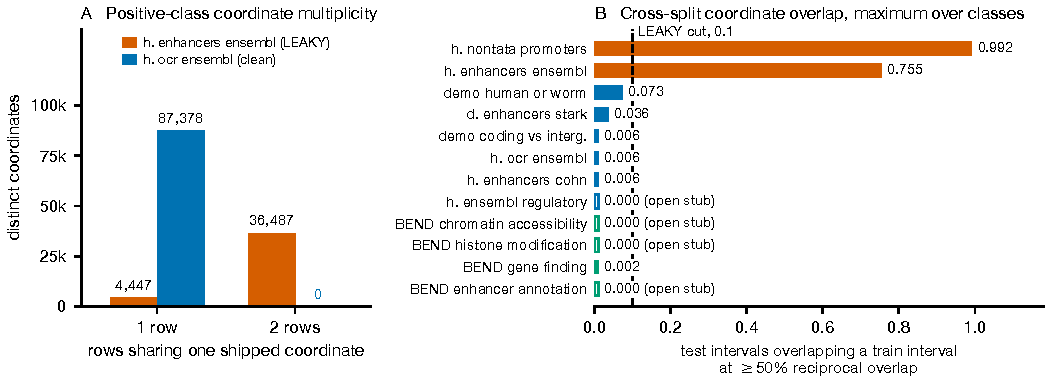
\includegraphics[width=\textwidth]{fig_coordinate_signature}
\caption{The construction defect in the shipped coordinates, measured before any model is trained. (A) Distinct positive-class coordinates by the number of rows sharing them, for the leaky \textit{human\_enhancers\_ensembl} and the clean \textit{human\_ocr\_ensembl}; $36{,}487$ of the former's coordinates carry two rows each, $94.3\%$ of its positive rows. (B) Fraction of test intervals overlapping any training interval at $\ge50\%$ reciprocal overlap, taken as the maximum over classes, for the eight Genomic Benchmarks datasets and the four BEND partitions (green); the dashed rule at $0.1$ is the LEAKY cut used throughout, carried over unchanged from sequence space, so the verdict cut adds no fitted parameter; the $\ge50\%$ overlap criterion is separately chosen (\S\ref{sec:m-coord}). A measured $0.000$ is drawn as an \emph{open} hairline stub and labelled as such, so that it is distinguishable both from a small non-zero bar and from a missing one; four of the twelve bars read exactly zero---\textit{human\_ensembl\_regulatory} and the three BEND partitions split by chromosome, BEND's identity-split gene-finding task reading $0.0017$. Overlap is strand-agnostic. \textit{demo\_coding\_vs\_intergenomic\_seqs} is the one miss: it is borderline in sequence space under containment, but one of its classes is keyed by transcript accession rather than by interval, so its $0.006$ is structurally zero rather than measured.\label{fig:coord}}
\end{figure*}



\subsection{Editing the construction step alone creates and cures the effect}\label{sec:r-manip}
Editing the construction step alone abolishes the syndrome in a leaky dataset and manufactures it in a clean one, turning the correlational coordinate evidence into a causal claim in both directions (Table~\ref{tab:manip}). Applying the omitted merge step to \textit{human\_enhancers\_ensembl}, at matched balance, collapses its leak fraction from $0.390$ to $0.012$ and the random-forest inflation from $+0.165$ $[0.157,0.173]$ to $-0.008$ $[-0.019,0.003]$---a null---and the reordering disappears, the forest sitting at rank~4 before and after correction. Imposing the same defect on the merged, clean \textit{human\_ocr\_ensembl}, at identical size \emph{and} balance, raises its leak fraction from $0.004$ to $0.204$ and its inflation from $+0.002$ $[-0.019,0.025]$ to $+0.105$ $[0.083,0.126]$, and manufactures the reordering: the forest is promoted to rank~1 on the contaminated split and demoted to rank~4 again by correction---the syndrome of \S\ref{sec:r-rank}, produced on demand. The effect is larger under matching than without it ($+0.063\to+0.105$), so the confounds were suppressing rather than creating it.

\begin{table}[tbp]
\begin{center}
\caption{Construct-and-break manipulations. Each intervention is paired with an unmanipulated control run of the identical pipeline at the same split seed and matched class balance; the break-a-clean pair is matched on size as well. Control rows are fresh seed-$0$ random splits, not the shipped partition. ``Leak'' is the near-duplicate test fraction at Jaccard $0.7$; ``Rank'' is the random forest before$\to$after correction, of four models. Intervals are two-arm cluster bootstraps over whole within-test components; $^{*}$ marks intervals excluding zero, and control and intervention intervals are disjoint in both directions.\label{tab:manip}}
\footnotesize\setlength{\tabcolsep}{1.5pt}\begin{tabular}{@{}llrrll@{}}
\toprule
& Condition & $n$ & Leak & RF drop [95\% CI] & Rank\\
\midrule
\multirow{2}{*}{Fix} & \textit{ensembl} control & 154{,}842 & 0.390 & $+0.165$ $[0.157,0.173]^{*}$ & $1\!\to\!4$\\
& \quad dup.\ collapsed & 81{,}868 & 0.012 & $-0.008$ $[-0.019,0.003]$ & $4\!\to\!4$\\
\midrule
\multirow{2}{*}{Break} & \textit{ocr} control & 20{,}000 & 0.004 & $+0.002$ $[-0.019,0.025]$ & $4\!\to\!4$\\
& \quad pos.\ duplicated & 20{,}000 & 0.204 & $+0.105$ $[0.083,0.126]^{*}$ & $1\!\to\!4$\\
\botrule
\end{tabular}
\end{center}
\end{table}

Duplicated rows scattered across a random split are leaky by construction; what the manipulation adds is that the full downstream syndrome, including the memorizer's promotion to rank~1, follows from the construction step alone. Size matching removes some of the duplicate partners it has just introduced, so the imposed leak fraction ($0.204$) is about half the undownsampled value ($0.498$) and the estimate is conservative. A ten-dose sweep on the same clean dataset, at one fit per dose, placed the first ranking inversion at an imposed leak fraction of $0.106$ and found none below it (Fig.~\ref{fig:manip}; Supplementary \S S2). Replication does not support that threshold, and we report the failure rather than the single-fit number: across $5$ split seeds $\times$ $3$ model seeds at each of the three doses bracketing the transition, inversion is a \emph{probabilistic} outcome whose rate rises from $0.60$ at $\varphi=0.088$ through $0.47$ at $\varphi=0.102$ to $0.87$ at $\varphi=0.116$, with split-clustered intervals that overlap across all three ($[0.27,0.93]$, $[0.07,0.87]$, $[0.60,1.00]$). Nine of the fifteen trials below the committed threshold inverted. Prediction P6---inversion above the diagnostic threshold and \emph{at none below}---is therefore refuted on replication, and no three-digit threshold is identifiable in this range; what survives is the monotone \emph{tendency}, not a breakpoint (Supplementary \S S2). Editing one curation step therefore both removes and installs the reordering, at a single fit per condition read only between arms.

\paragraph{Replication: a design, not an anecdote.} Repeating break-a-clean on two further
clean donors, with nothing retuned, the manufactured \emph{inflation} replicates on all three: at
matched size and balance both \textit{human\_enhancers\_cohn} and \textit{drosophila\_enhancers\_stark}
move from a control whose forest-drop interval includes zero to a manipulated arm whose interval
excludes it ($+0.076$ and $+0.066$). The manufactured \emph{reordering} replicates on two of three,
and the exception is informative: on \textit{drosophila\_enhancers\_stark} the forest is already
rank~4 as shipped, so no demotion is available for the defect to produce. Imposing this construction
reliably inflates a memorization-prone model; whether it also reorders depends on where that model
started. A size-matched control for the fix-a-leaky direction rules out the training-set size
difference as the explanation. Full arms: Supplementary \S S6.

\begin{figure}[tbp]
\centering
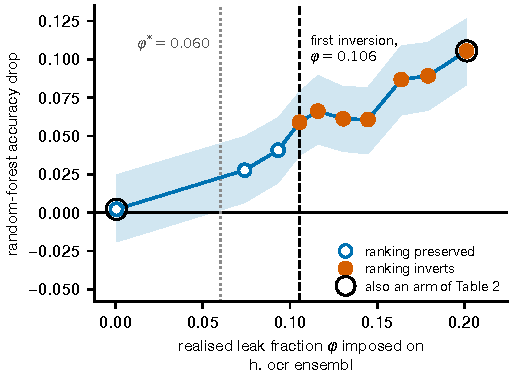
\includegraphics[width=\columnwidth]{fig_manipulation}
\caption{Ten doses of the same construction defect, imposed on the clean \textit{human\_ocr\_ensembl}. Random-forest accuracy drop under near-duplicate-aware correction against the realised test-set leak fraction $\varphi$ at Jaccard $0.9$; the shaded band is the two-arm cluster-bootstrap $95\%$ CI over whole within-test near-duplicate components, and each dose is a single fit at one split seed. Filled points are doses at which the four-model ranking inverts, open points doses at which it does not. Circled points are the two arms of Table~\ref{tab:manip} re-reported rather than fresh trials, so the sweep supplies eight additional doses. The dashed rule marks the first inversion, the dotted rule the diagnostic threshold $\varphi^{*}$ computed at that dose.\label{fig:manip}}
\end{figure}

\subsection{What a near-duplicate-aware split costs, and where the cost comes from}\label{sec:r-drop}
Under the re-split the best model's accuracy drops sharply on the leaky datasets and nowhere else: $16.5$ points on \textit{human\_enhancers\_ensembl} ($0.8596\to0.6951\pm0.0019$ over five re-split seeds; combined-source Wald CI $[15.4,17.4]$) and $11.8$ on \textit{human\_nontata\_promoters} ($0.9284\to0.8101\pm0.0055$). On that second dataset the point estimate and the interval are computed on different estimands, so both are named: $11.8$ points is the five-seed mean, while the combined-source interval $[8.7,13.0]$---which folds in re-split-seed variance exactly as the \textit{human\_enhancers\_ensembl} figure above does---is computed on the seed-$0$ partition, where the delta is $10.8$ points; the cluster bootstrap alone gives $[9.2,12.6]$. Every clean-dataset delta includes zero for the memorizing forest as well as the linear models, the largest being \textit{drosophila\_enhancers\_stark} at $+0.024$, cluster-bootstrap CI $[-0.007,0.054]$. The negative control confirms causation: a random re-split at matched size and balance leaves the leaky-dataset accuracies unchanged (best-model deltas $-0.001$ and $-0.002$, point estimates, two orders of magnitude below $0.118$ and $0.165$; Supplementary Fig.~S1), so only removing near-duplicates, not re-splitting per se, lowers the score. Corrected accuracy is stable across five re-split seeds and, independently, five forest training seeds ($0.698\pm0.002$; $0.821\pm0.003$), the forest demoted on every seed. That de-leaking lowers apparent accuracy is established across domains \citep{kapoor2023leakage,rafi2026,bushuiev2024}; what the within-suite version adds is the matched clean control, on which the same procedure moves nothing.

\paragraph{Two effects, separated.} That drop conflates two quantities a single number hides, and a third arm separates them: one fit on the as-shipped training set, scored twice---on the whole as-shipped test set and on its \emph{novel} stratum alone (Table~\ref{tab:decomp}). \textbf{Evaluation-side inflation}, what the benchmark overstates about a model that already exists, needs no re-splitting and no retraining and accounts for $8.98$ of the forest's $16.4$ points ($0.8596\to0.7698$, cluster-bootstrap $[8.7,9.3]$). \textbf{Split-side effect}, the retraining penalty from stripping near-duplicate partners out of training too, accounts for the remaining $7.41$ ($0.7698\to0.6957$). Both are large, and the split-side half is not a measurement error at all. On \textit{human\_nontata\_promoters} the same decomposition gives $4.91$ and $6.64$ points.

Two features of this decomposition matter more than its headline. First, the split side is where the memorizer is singled out: on \textit{human\_enhancers\_ensembl} it is the \emph{only} model of the four that pays a retraining penalty, the three others gaining slightly when refit on de-leaked data ($-0.013$, $-0.013$, $-0.009$), so the ranking change is not a rising tide. Second, the novel stratum is not class-balanced like the full test set ($0.197$ positive against $0.500$; $0.982$ against $0.544$ on \textit{human\_nontata\_promoters}), so the raw evaluation-side figure is prevalence-confounded in the same way \S\ref{sec:r-mech}'s raw gap is---a constant classifier scores $+0.303$ and $-0.438$ on it for free. From balanced accuracy, for which a constant classifier scores zero, the forest's evaluation-side inflation is $+0.1789$ and $+0.1452$, and the linear models' $+0.0320$ to $+0.1156$---the top of that range being \textit{LinearSVC} on \textit{human\_nontata\_promoters}, which is the one linear cell that approaches the forest's. Separately from either effect, the ranking on the novel stratum has \emph{already} changed under the as-shipped fit, the forest scoring $0.770$ against \textit{LinearSVC}'s $0.782$---a margin of $1.2$ points, which is a different quantity from the $8.98$ above and was previously reported in a way that invited the two to be confused.

\begin{table*}[tbp]
\begin{center}
\begin{minipage}{\textwidth}
\caption{Three-arm decomposition of the corrected-split drop. \textbf{As-shipped} and \textbf{Novel-only} are the \emph{same fitted model}---one fit on the as-shipped training set---scored on the whole as-shipped test set and on its novel stratum alone (maximum $8$-mer Jaccard to any training sequence $<0.5$). Their difference is \textbf{evaluation-side inflation}: it requires neither re-splitting nor retraining, and is what the benchmark overstates about a model that already exists. \textbf{Corrected} refits on the near-duplicate-aware split, and its difference from Novel-only is the \textbf{split-side effect}, a retraining penalty rather than a measurement error. The two sum to the total drop. Only the random forest pays a split-side penalty on \textit{human\_enhancers\_ensembl}; the other three improve slightly when refit on de-leaked data. Corrected accuracies here are means over the three re-split seeds this decomposition run used, not the five the headline drop uses, which is why the forest reads $0.6957$ in this table and $0.6951$ in \S\ref{sec:r-drop}; the two conventions differ by $0.0006$ on this dataset and no conclusion turns on which is quoted. The novel stratum's class balance differs from the full test set's ($0.197$ against $0.500$ here), so these raw figures are prevalence-confounded and the balanced-accuracy versions are given in the text.\label{tab:decomp}}
\resizebox{\textwidth}{!}{% GENERATED by audit/pipeline/emit_tables.py -- do not edit by hand.
% Edit the source CSV and re-run, or the next build will overwrite you.
\begin{tabular}{@{}llrrrrrr@{}}
\toprule
Dataset & Model & As-shipped & Novel-only & Corrected & Eval-side & Split-side & Total\\
 &  & (full test) & (same fit) & (re-split) & inflation & effect & drop\\
\midrule
human\_enhancers\_ensembl & RandomForest & 0.8596 & 0.7698 & 0.6957 & $+0.0898$ & $+0.0741$ & $+0.1639$\\
 & LinearSVC & 0.7980 & 0.7820 & 0.7952 & $+0.0160$ & $-0.0132$ & $+0.0028$\\
 & LogisticReg. & 0.7809 & 0.7649 & 0.7776 & $+0.0161$ & $-0.0127$ & $+0.0033$\\
 & HistGB & 0.7636 & 0.7488 & 0.7574 & $+0.0148$ & $-0.0086$ & $+0.0063$\\
\midrule
human\_nontata\_promoters & RandomForest & 0.9284 & 0.8793 & 0.8129 & $+0.0491$ & $+0.0664$ & $+0.1155$\\
 & LinearSVC & 0.8876 & 0.8546 & 0.8063 & $+0.0331$ & $+0.0482$ & $+0.0813$\\
 & LogisticReg. & 0.8702 & 0.8340 & 0.8300 & $+0.0361$ & $+0.0041$ & $+0.0402$\\
 & HistGB & 0.8905 & 0.8383 & 0.8244 & $+0.0523$ & $+0.0139$ & $+0.0661$\\
\botrule
\end{tabular}
}
\end{minipage}
\end{center}
\end{table*}

\subsection{The shipped split distorts model comparison, and can invert it}\label{sec:r-rank}
\paragraph{The four-model comparison.} On \textit{human\_enhancers\_ensembl} the best model \emph{changes}. In the four-model comparison the near-default random forest, ranked first as shipped ($0.860$), falls to last after correction ($0.696$) and \textit{LinearSVC} becomes best ($0.798$; Fig.~\ref{fig:ranking}). This holds under accuracy, AUROC ($0.805$ against $0.870$) and $F_1$ ($0.635$ against $0.796$), so it is not a threshold artifact; the bootstrap probability that the forest ranks first goes from $1.0$ to $0.0$; and it reproduces under the chromosome-holdout control (\S\ref{sec:r-robust}).

\paragraph{Nine learners: a tie as shipped, $23$ points corrected.} Widening from four learners to nine sharpens the statement (Supplementary Table~S2). The as-shipped split does not separate its top three: the MLP ($0.8736$), $1$-nearest-neighbour ($0.8729$) and extremely randomized trees ($0.8721$) finish within $0.0015$, and the paired interval on the top-two margin, $[-0.005,0.006]$, includes zero. On the corrected split those three span $23$ accuracy points ($0.768$, $0.537$, $0.628$). The distortion is therefore not only that a different model is crowned; three learners the shipped split reports as tied are $23$ points apart once the near-duplicates are removed. Two controls bound how much of that separation is real, and they do not agree, so we report both and weaken the claim accordingly.

The first is a clean-dataset control, since the registered P4 governs \emph{drops} rather than spread. Running the same nine-model roster and the same whole-cluster re-split on two clean datasets, top-three spread does not expand: on \textit{human\_enhancers\_cohn} it goes $0.0218$ $[0.0120,0.0328]$ as shipped to $0.0210$ $[0.0102,0.0318]$ corrected, and on \textit{demo\_human\_or\_worm} it \emph{contracts}, $0.0086$ $[0.0050,0.0134]$ to $0.0056$ $[0.0026,0.0104]$. Re-splitting alone therefore does not manufacture spread.

The second control is harsher and is the one that constrains the claim. Top-$k$ spread also expands mechanically as an operating point falls away from a ceiling, independently of whether the underlying differences are real. Re-weighting the \emph{as-shipped} test set on a held-out difficulty panel until the same three models average the corrected split's accuracy ($0.6951$), and changing nothing else---no re-split, no retraining---their spread expands from $0.0015$ to $0.1424$ $[0.1373,0.1483]$. That is most of the way to the corrected split's $0.2314$. Difficulty alone therefore accounts for the majority of the expansion, and only the excess above it---roughly $0.09$ of the $0.23$---is attributable to de-leaking. We accordingly claim that correcting the split separates models the as-shipped benchmark reports as tied, by more than a difficulty-matched test set of the same accuracy would, and not that the full $23$ points measures real model quality. The matched draw is also slightly \emph{more} near-duplicate-rich than the full test set ($0.406$ against $0.380$ at Jaccard $\ge0.9$), which if anything understates the difficulty effect. \textit{human\_nontata\_promoters} sits between the regimes at $0.0345\to0.0898$. The linear SVM rises from rank~5 to~1 and logistic regression from~6 to~2, while $1$-nearest-neighbour falls from rank~2 to~9, last, at $0.537$---$3.7$ points above the $0.500$ base rate of this balanced test set, on $n=30{,}971$. The two models exchanging the top slot each lead on their own split by a paired margin excluding zero ($[0.071,0.080]$ as shipped, $[0.024,0.035]$ corrected). The four models whose drops exclude zero are $1$-NN, the forest, extremely randomized trees and the MLP; the other five---both linear models, boosting, naive Bayes and $15$-nearest-neighbour, which we designated memorization-prone in advance---are null. The MLP is not one of those four designated learners, so its presence says the inflation reaches a neural learner too.

\begin{figure*}[tbp]
\centering
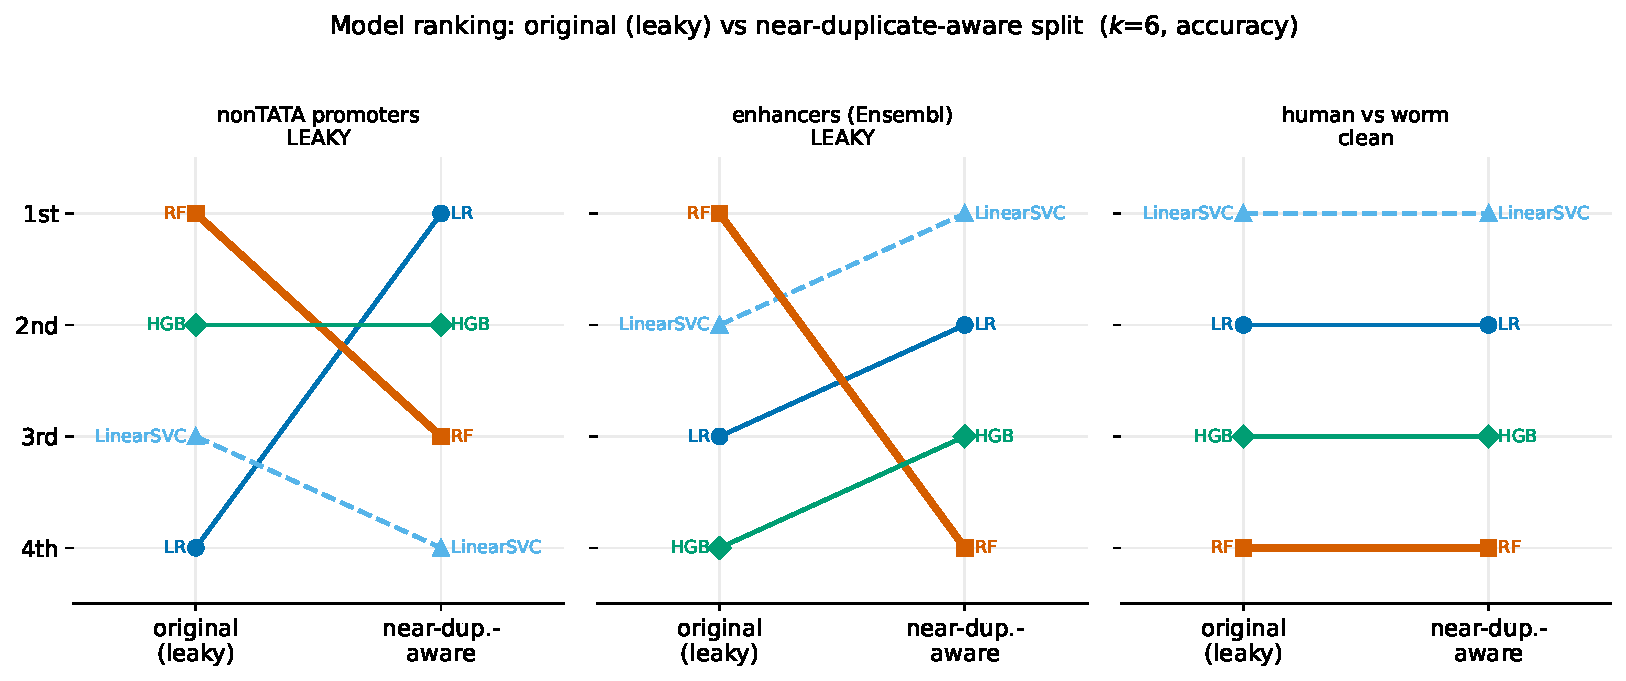
\includegraphics[width=\textwidth]{fig_ranking_inversion}
\caption{Four-model rankings on the original (leaky) split versus the near-duplicate-aware split ($k$=6, accuracy). The random forest is dethroned on \textit{human\_enhancers\_ensembl} (middle) and, under accuracy only, on \textit{human\_nontata\_promoters} (left), while rankings are stable on the clean control \textit{demo\_human\_or\_worm} (right, $20$k subsample). Kendall $\tau$ is deliberately not annotated: at four models it is too coarse to carry (\S\ref{sec:r-rank}), and it orders these panels opposite to the conclusions they support.}\label{fig:ranking}
\end{figure*}

\paragraph{A convolutional network, not only trees.} The result above rests on a tree ensemble, so the natural objection is that it is an artifact of one model family. It is not, and the test uses the architecture this suite itself baselines \citep{gresova2023}: a 1D residual CNN trained from scratch on each training split, carrying no pretraining confound. The leaky split ranks it fifth of ten; the corrected split ranks it first, on each of five training seeds. The registered nine are unaffected by adding it---the linear SVM remains the corrected winner \emph{of the registered nine}---and the CNN is a tenth, \emph{post hoc} entrant. Replicating the pre-registered reference cell across five training seeds on the same corrected partition gives corrected accuracies $0.8028$--$0.8131$ (mean $0.8086$, sd $0.0040$) against the linear SVM's $0.7975$, and as-shipped accuracies $0.8119$--$0.8359$, between the forest's $0.8596$ and the linear SVM's $0.7980$, so the rank is the same on every seed. The exchanging pair is the MLP and the CNN, and both arms of the inversion criterion clear zero: as-shipped MLP$-$CNN $+0.0500$ $[0.0320,0.0679]$, corrected CNN$-$MLP $+0.0402$ $[0.0309,0.0495]$. Against the harder comparator the criterion does not require, \textit{LinearSVC}, the paired difference is $+0.0111$ with a combined-source interval of $[0.0019,0.0204]$, folding the seed-to-seed standard deviation ($0.0040$) into the cluster-bootstrap standard deviation ($0.0026$) in quadrature, because the quantity of interest is the advantage of \emph{one} trained network rather than of an average over five. Bootstrapping seed-averaged per-example correctness instead gives $[0.0063,0.0161]$, narrower than any individual seed's interval because averaging removes the training variance rather than estimating it, and we do not quote that as the result. Four of the five individual seeds have paired intervals excluding zero and the fifth does not ($+0.0053$, $[-0.0006,0.0109]$), so against that harder comparator the advantage is uniform in rank across seeds but not uniform in significance; we report the per-seed intervals rather than an average that would conceal the spread. The corrected advantage over \textit{LinearSVC} is also an order of magnitude smaller than the forest's inflation---roughly $1$ point against $16$---so the CNN corroborates the mechanism in a second model family and does not carry the headline on its own. The reference cell is the \emph{maximum} of the nine-cell regularization grid, whose corrected accuracies span $0.749$--$0.813$ with $0.7975$ inside---five cells above, four below---so no conclusion is drawn from that cell alone; the claim rests on seed replication of one pre-specified cell against a paired interval.

\paragraph{The second leaky dataset: a negative result.} On that dataset the picture is weaker, and we report it as a failure of the claim rather than as a second demonstration of it. Under accuracy the forest is demoted from rank~1 to~3 (corrected LR $0.829>$ HGB $0.827>$ RF $0.820>$ LinearSVC $0.808$, all seed-$0$; the forest's $0.820$ is the seed-$0$ value of the quantity whose five-seed mean, $0.810$, gives the headline drop). This is a statistical dead heat---corrected CIs overlap (RF $[0.812,0.828]$, LR $[0.821,0.837]$)---and does not survive a threshold-free metric: under AUROC and $F_1$ the forest remains rank~1 (corrected AUROC $0.929$, highest of the four). With only four models Kendall $\tau$ is too coarse for a primary statistic. The nine-model roster produces a larger scramble there with supported swap margins, but the prevalence-corrected graded gap does not separate the model families on it (memorizers $+0.122$ against $+0.179$), so the wider roster does not strengthen that dataset's case; an alternative discriminator fails too, the residual of each drop against $\varphi g$ being \emph{larger} on \textit{human\_enhancers\_ensembl} ($+0.257$) than on \textit{human\_nontata\_promoters} ($+0.152$), so it measures the retraining penalty rather than dataset quality. The reordering therefore stands as an existence proof on \textit{human\_enhancers\_ensembl} and as a cautionary partial case on \textit{human\_nontata\_promoters}.

\paragraph{Scope: what the ranking result claims, and what it does not.} Three conditions are jointly necessary for the inversion, and each is measured here rather than assumed. \emph{(i)} A memorization-prone learner must be in the comparison set. The effect lives at \texttt{min\_samples\_leaf}$=1$ and has gone by $20$ (\S\ref{sec:r-mech}); that configuration is not a strawman a careful practitioner would avoid, because ordinary stratified cross-validation on the as-shipped training set selects it and the benchmark then rewards it. \emph{(ii)} A challenger must be genuinely better on novel sequences. The Nucleotide Transformer tasks supply leakage without one, and no ranking there inverts (\S\ref{sec:r-census}). \emph{(iii)} The construction must leave near-duplicates spanning the split (\S\ref{sec:r-manip}). Given all three, the reordering appears on one shipped dataset, is manufactured to order on two of three independent clean donors, and is absent from the second shipped leaky dataset under any threshold-free metric. The claim we make is therefore that the shipped split can materially distort model comparison and invert it under stated conditions---not that this benchmark is unable to rank models in general, which the evidence here does not support.

\paragraph{The six registered predictions, scored.} Six predictions were committed in code, inside the module that would test each, before that module was run; all six are scored whether or not they held (Table~\ref{tab:prereg}), with their verbatim text in Supplementary \S S1.9. Two hold outright, two hold on \textit{human\_enhancers\_ensembl} and not on \textit{human\_nontata\_promoters}, one fails as registered and one is refuted on replication.

\begin{table*}[tbp]
\begin{center}
\begin{minipage}{\textwidth}
\caption{The six predictions committed in code before the module testing each was run, scored. Outcomes are reported against the statistic each prediction named at registration, not against a later reformulation of it. \emph{ens.}~is \textit{human\_enhancers\_ensembl} and \emph{nont.}~is \textit{human\_nontata\_promoters}.\label{tab:prereg}}
\footnotesize\setlength{\tabcolsep}{4pt}\begin{tabular}{@{}llp{0.30\textwidth}p{0.42\textwidth}@{}}
\toprule
& Outcome & Registered claim & Scored against\\
\midrule
P1 & Fails & $1$-NN carries the largest \emph{raw} graded memorization gap & The largest raw gap is the forest's on ens.\ ($0.230$, against $1$-NN's $0.208$ and extremely randomized trees' $0.210$) and $15$-NN's on nont. Under the prevalence-corrected gap $1$-NN does lead on ens.\ ($+0.461$ against $+0.319$), but that statistic was defined after P1 was committed, so the reading is \emph{post hoc} and is not counted as a confirmation.\\
P2 & Holds on ens.\ only & $1$-NN carries the largest split-induced drop & Largest of the nine on ens.\ ($0.336$); fails on nont., where P1 fails as well.\\
P3 & Holds & The four memorization-prone learners outrank the two linear models as shipped and fall below them once corrected & Mean rank $4.50$ against $5.50$ as shipped and $7.25$ against $1.50$ corrected, on ens.\\
P4 & Holds & On a clean control no model's drop interval excludes zero & True for all nine on \textit{human\_enhancers\_cohn}. That control runs on a $20{,}000$-sequence subsample rather than the full $27{,}791$, admissible because its full-scale leak fractions are $0.001$ and $0.005$.\\
P5 & Holds on ens.; tie on nont. & Cluster-grouped cross-validation selects a more regularized forest than naive cross-validation & On ens.\ cluster-grouped cross-validation selects \texttt{min\_samples\_leaf}$=20$ where the naive procedure selects $1$; on nont.\ both select $1$, which is a tie and not a reversal (\S\ref{sec:r-mech}).\\
P6 & Refuted on replication & A ranking inversion occurs at every imposed leak fraction above the diagnostic threshold and at none below & The ten single-dose fits agree, but across $5$ split seeds $\times$ $3$ model seeds at the three doses bracketing the transition, inversion is probabilistic ($0.60$, $0.47$, $0.87$) with overlapping intervals, and nine of the fifteen trials below the threshold inverted (\S\ref{sec:r-manip}; Supplementary \S S2).\\
\botrule
\end{tabular}
\end{minipage}
\end{center}
\end{table*}

\subsection{Which learners, and which configurations, carry the effect}\label{sec:r-mech}
\paragraph{The mechanism.} On \textit{human\_enhancers\_ensembl} the near-default forest scores $1.000$ on near-duplicate test sequences ($\ge0.9$ similarity) but $0.770$ on novel ones---a raw graded gap of $+0.230$ against $0.034$--$0.037$ for the other three learners of the four-model comparison, though across the wider roster the raw gaps reach $0.210$ and $0.208$. On novel sequences the forest ($0.770$) is in fact \emph{worse} than the linear SVM ($0.782$). Those are the registered quantities, and on them P1 fails.

\paragraph{Exploratory, and reported as such.} P1 was committed against the \emph{raw} graded gap
and fails on it. A prevalence-corrected form of the statistic, defined afterwards, does separate the
model families on \textit{human\_enhancers\_ensembl}, $1$-nearest-neighbour carrying the largest gap
and the four memorization-prone learners averaging above the other five, and does \emph{not} on
\textit{human\_nontata\_promoters}, which is why the mechanism claim is scoped to the first dataset.
Because that statistic was defined after the prediction it rescues, it cannot confirm the hypothesis
and is registered forward instead: on the next leaky dataset audited, $1$-nearest-neighbour will
carry the largest corrected gap and the memorization-prone four will average a larger one than the
remaining five. The shape of accuracy against similarity, and how it compares with the non-monotonic
curve \citet{rafi2026} report, is likewise exploratory. Both are in Supplementary \S S10.

\paragraph{The effect requires the unregularized forest.}\label{sec:r-regpath} At \texttt{min\_samples\_leaf=1} the forest scores exactly $1.000$ on the $\ge0.9$ bin, with drops of $0.164$ and $0.108$ (seed $0$), graded gaps $0.230$ and $0.121$, and rank~1. At $500$ the drop is $\approx0$ ($0.164\to-0.001$; $0.108\to0.000$) and the leaf-size gap collapses ($0.230\to0.020$; $0.121\to0.061$), monotonically but for one $0.0012$ reversal in the last \textit{human\_nontata\_promoters} step; along the depth axis the gap is non-monotone there, rising to $0.224$ at depth $16$ before falling to $0.161$. Crucially, the ``forest wins on the leaky split'' phenomenon itself \emph{requires} the unregularized forest: as shipped it holds rank~1 only near the default and has fallen to rank~4 by \texttt{min\_samples\_leaf}$\ge20$ on both datasets. Regularization removes the inflation without recovering the accuracy the inflation concealed---corrected accuracy on \textit{human\_nontata\_promoters} falls $0.820\to0.785$ along the same path---so the two interventions are not interchangeable.

\paragraph{Ordinary tuning selects that configuration.}\label{sec:r-tuning} A practitioner does not know a split is leaky; they tune by cross-validating on the training set. On \textit{human\_enhancers\_ensembl}, ordinary stratified $5$-fold selects \texttt{min\_samples\_leaf}$=1$, the memorizing default, and the model it selects scores $0.860$ as shipped but $0.696$ corrected---a loss of $16.4$ points. Cluster-grouped $5$-fold selects $20$, and that model loses only $2.2$ points ($0.751\to0.729$). Worse, the benchmark punishes the correct methodology: the leakage-aware tuner's model appears $10.9$ points \emph{worse} as shipped ($0.751$ against $0.860$) while being $3.3$ points \emph{better} corrected ($0.729$ against $0.696$)---a point-estimate comparison to which we attach no interval. On \textit{human\_nontata\_promoters} both procedures select $1$, so P5 holds on the first dataset and is a tie, not a reversal, on the second. The untuned default is therefore not a careless choice a tuner would correct; it is what ordinary model selection selects, and the benchmark rewards it.

\paragraph{Deep models, binary and multiclass.}\label{sec:r-deep} A from-scratch 1D CNN trained only on each training split shows the same inflation, so the effect is not a classical-model artifact. The pre-registered reference cell drops on \emph{both} datasets---$+0.043$ on \textit{human\_nontata\_promoters} $[0.025,0.061]$, $+0.014$ on \textit{human\_enhancers\_ensembl} $[0.007,0.021]$---so the refutation condition, which requires the interval to include zero on \emph{both}, is not triggered. One \textit{human\_enhancers\_ensembl} seed does include zero, and \textit{human\_nontata\_promoters}, which carries the larger drop, was not seed-replicated and is the more dispersed of the two across the grid, so the verdict rests on an unreplicated cell on the dataset from which \S\ref{sec:r-mech} scopes the mechanism away. Nineteen of $20$ cells drop with intervals excluding zero; the exception is the \textit{human\_nontata\_promoters} dropout-$0.6$ cell, where accuracy \emph{rises} $0.020$. Seed replication of the \textit{human\_enhancers\_ensembl} reference cell gives drops of $0.0049$--$0.0269$, a five-fold spread whose smallest does not exclude zero, so $+0.014$ is one draw and no single-run drop here, including each of the nineteen, is a point estimate. One registered expectation was not met: the pre-registration named this a \emph{dose-response} grid, and it is not one, the drop being non-monotone in both dropout and weight decay.

The multiclass question is answered by construction, and the two model families answer it differently. On the identical injected construction the forest's drop grows monotonically with $f$: $+0.0004$, $+0.1177$, $+0.1791$, $+0.2581$ at $f=0$, $0.1$, $0.2$, $0.4$. Logistic regression is not untouched---it drops $0.0158$, $0.0323$, $0.0661$, monotone in $f$, its as-shipped accuracy climbing $0.591\to0.669$ as it exploits the injected copies---but the forest's advantage is $7.4\times$ to $3.9\times$ larger, narrowing as the dose rises. The CNN shows \emph{no} dose-response: mean drops $-0.0386$ (sd $0.0239$), $-0.0182$ ($0.0296$), $-0.0249$ ($0.0325$), $-0.0089$ ($0.0362$) over three seeds at the same four doses (each cell a single run)---every mean negative, the seed standard deviation equalling or exceeding any dose effect. All three seeds are reported; seed $1$ underfits, its as-shipped accuracy averaging $0.6856$ against $0.7552$ and $0.7534$, and is retained rather than excluded. The mechanism therefore generalizes to multiclass \emph{for the classical memorizer} and not for the regularized network---what ``memorization propensity, not capacity'' predicts, since the label-carrying copies are available to every learner and the differential is a property of which learner exploits them.

\subsection{Beyond the suite: a second census, and a falsified prediction}\label{sec:r-census}
\paragraph{The Nucleotide Transformer tasks: three of eleven are leaky, and no ranking inverts.} Counting independent tasks, three of eleven Nucleotide Transformer tasks are leaky and six more borderline, leaving two clean. \textit{enhancers} carries $25.0\%$ test-to-train leakage that is \emph{byte-identical}---verified on a code path using no $k$-mers, $100$ of $400$ test sequences at label concordance $1.000$---while \textit{splice\_sites\_acceptors} and \textit{\_donors} carry $0.244$ and $0.245$ at Jaccard $0.7$ with zero exact duplicates. An earlier pass capped training sets at $20{,}000$ and returned three borderline and five clean; re-running uncapped moved three histone tasks across the cut on containment.

The splice mechanism is not the cross-species homology an earlier account proposed: $65.9\%$ and $68.3\%$ of leaked test sequences share the same UniProt entry name with their best training partner---same gene, same organism---and at Jaccard $\ge0.9$ that share \emph{rises} to $77.1\%$ and $82.6\%$, where homology predicts thinning. It is same-gene splice-window redundancy, and label concordance among leaked pairs is correspondingly poor ($0.819$, $0.792$ against $0.999$ on both Genomic Benchmarks datasets). That account is offered after the fact, not predicted (Supplementary \S S3).

Running the full pipeline there returns a null: no material ranking inversion on any leaky task nor on the control. Leakage does inflate scores on \textit{enhancers}---the forest drops $0.0413$ $[0.0241,0.0583]$, \textit{LinearSVC} $0.0221$ $[0.0055,0.0381]$, HistGradientBoosting $0.0185$ $[0.0021,0.0366]$, three of the four learners excluding zero, while logistic regression, leading on both splits, is null ($+0.0046$ $[-0.0104,0.0199]$). The memorization \emph{ordering} reproduces---the forest carries the largest drop and is the only learner with a positive graded gap ($+0.100$ against $-0.084$ to $-0.169$)---but the confinement to memorizers reported on \textit{human\_enhancers\_ensembl} does not: two non-memorizers exclude zero here, and their negative graded gaps rule out memorization, leaving the retraining penalty of \S\ref{sec:r-rank} the better reading. On \textit{splice\_sites\_acceptors} the memorizing forest's drop is null ($+0.0201$ $[-0.0068,0.0446]$), so the model carrying the mechanism is the one the effect does not reach. On \textit{splice\_sites\_donors} correction \emph{raises} accuracy for three of four learners and one gain is nominally supported (\textit{LinearSVC} $-0.0251$ $[-0.0526,-0.0004]$), marginally and seed-dependently ($p\approx0.059$ uncorrected). Under Benjamini--Hochberg across this cross-suite grid only \textit{enhancers}$|$RF survives, so these flags are nominal---with one qualification that runs against us and is therefore reported: under a single pooled family of all $31$ deltas (\S\ref{sec:r-robust}) \textit{enhancers}$|$LinearSVC survives as well, at $q=0.049$, close enough to the cut that the normal approximation behind these $p$-values cannot resolve it either way. The leading model is unchanged on all four tasks, which is the claim this section rests on: reordering additionally requires a challenger genuinely better on novel sequences, and this suite supplies leakage without one.

\paragraph{GUE: a pre-registered prediction, falsified.}\label{sec:r-gue} Our pre-registration carried binding predictions for GUE \citep{zhou2023dnabert2}, recorded before that suite was examined---the prediction document was committed as \texttt{2edad5c} on 2026-07-18 and the census that scored it as \texttt{3af3eb4} nine hours later, in separate commits whose ordering is published with the \texttt{git log} output in \texttt{PREREGISTRATION.md}, subject to the limits of author-controlled timestamps stated there: that its short fixed-length human regulatory tasks---core promoter at $70$\,bp, promoter at $300$\,bp, transcription-factor binding at $101$\,bp---would be leaky, and its multi-species tasks clean. At full scale the registered predictions score $3$ of $15$, and all eleven predicted-leaky tasks are clean, measuring $0.009$ to $0.041$ under Jaccard and $0.014$ to $0.042$ under containment---little leakage, not none, the largest under half the verdict cut. These are not eleven independent benchmarks: the \textit{\_all} promoter tasks' test sets are the exact union of their own \textit{notata} and \textit{tata} test sets, and the $70$ and $300$\,bp promoter families are the same loci at two window widths, leaving seven independent test partitions, which bounds how much independent evidence the null carries.

This refutes the hypothesis the prediction encoded. Leakage does not track task type: seven independent benchmarks in precisely the regime we flagged do not carry it. What it tracks is the construction step of \S\ref{sec:r-coord}---Genomic Benchmarks' two leaky datasets have an un-deduplicated assembly where GUE's comparable tasks do not. Two verdicts moved. \textit{emp\_H3K4me3}, registered clean, has a full-scale containment leak fraction of $0.138$ against $0.093$ capped, making it borderline: under the binary rule committed in advance it remains a correct prediction and the score stands at $3$ of $15$; under a three-way rule it is a miss and the score is $2$ of $15$. And \textit{virus\_covid}, also registered clean, measures $1.000$---the twelfth miss, and the one discussed in \S\ref{sec:d-detector}, where it is not a curation defect. Overall, the prediction that leakage follows task type is refuted by seven independent partitions in precisely the regime it named; the two verdicts that moved are borderline calls, not reversals.

\subsection{Robustness}\label{sec:r-robust}
Six robustness arms are reported in full in Supplementary \S S7, and none moves a verdict or an
interval. The block bootstrap confirms the dependence is real and \emph{larger} than a mean-size
design effect suggests---Kish's $m^{*}$ is $4.45$ and $2.58$ where the mean block is $1.55$ and
$1.33$---and is concentrated in the corrected arm the splitter creates, yet it is already inside
every reported interval because that is the unit those intervals resample; the forest's drop still
excludes zero on both datasets. The chromosome-holdout control reproduces the demotion on
\textit{human\_enhancers\_ensembl} (rank~$1\to4$) and does \emph{not} on
\textit{human\_nontata\_promoters}, a third independent signal that the latter's demotion is
accuracy-only. The effect survives canonical $k$-mer features, a GC-in-distribution restriction and
an MMseqs2 alignment-scored re-clustering, and cluster cohesion explains the asymmetry between the
two datasets geometrically rather than biologically, the two sitting an order of magnitude either
side of the correction-safety cut. Pooling both
multiplicity families into one changes no conclusion and adds one flag. Against hashFrag
\citep{rafi2026}, the closest runnable comparator, a threshold window reproduces $7$ of our $8$
verdicts, and the single disagreement---\textit{drosophila\_enhancers\_stark}---marks the boundary
between near-duplication and homology rather than an error in either tool. Under induced prevalence
imbalance, AUPRC and MCC fall several times further than accuracy on both datasets, so accuracy at
threshold $0.5$ understates the correction.

\section{Discussion}\label{sec:discussion}

Near-duplicate leakage in this suite is produced by a step in how the data were assembled, and that step is visible, editable and reversible before any model is trained: a coordinate signature carrying no sampling uncertainty and no model dependence, a manipulation that removes and imposes the defect at will, and a pre-registered task-type prediction that failed on all eleven targets. On one dataset the downstream cost is a change in which model the benchmark reports as best.

The reordering requires the \emph{unregularized} forest, which by \texttt{min\_samples\_leaf}$\ge20$ has already fallen to rank~4 as shipped (\S\ref{sec:r-regpath}). That configuration is not a careless choice a practitioner would correct: ordinary stratified cross-validation on the as-shipped training set selects it, and the benchmark then penalises the practitioner who tunes correctly, showing the leakage-aware tuner's model $10.9$ points worse as shipped and $3.3$ points better corrected (\S\ref{sec:r-tuning}). What matters in a benchmark is not whether some user tunes but whether the data reward memorization at all. The controlled variable is memorization propensity rather than capacity: the higher-capacity HistGradientBoosting is barely inflated where the near-default forest is heavily inflated, and the regularized CNN shows no dose-response under injection at all (\S\ref{sec:r-deep}).

The suite's own published baseline is a convolutional network \citep{gresova2023}, not a tree ensemble. A CNN-based leaderboard is affected in the direction that costs the architecture: our from-scratch network ranks fifth of ten as shipped and first corrected, scoped to one dataset and to a \emph{post hoc} comparison, with one of its five seeds not individually clearing zero (\S\ref{sec:r-rank}). Its inflation is six- to thirtyfold smaller than the forest's depending on seed, the reordering condition is not met by a CNN-only comparison, and the result is bounded by its comparison set: ten learners, one dataset.

One interpretive point governs every corrected number in this paper. A near-duplicate-aware split answers how a model scores on test sequences with no near-copy in training, which is not how a deployed model will perform---paralogues, gene families and conserved regulatory elements are real inputs---and whole-cluster assignment also strips near-duplicate partners from the \emph{training} set. ``Corrected'' therefore qualifies the split and not the accuracy: the as-shipped ranking is wrong, and the corrected accuracy is a lower bound under one adversarial notion of novelty, not a deployment estimate.

\textit{human\_enhancers\_ensembl} is an existence proof: the ranking change holds under accuracy, AUROC, $F_1$, a bootstrap winner probability, a chromosome-holdout control and an alignment-scored re-clustering. It is one instance among shipped datasets, and we do not present it as more; but it is not alone once the construction step is treated as an experimental variable, the same reordering being manufactured on two of three independent clean donors and the third explained rather than excused---its memorizer already ranked last, so no demotion was available (\S\ref{sec:r-manip}). One in-the-wild instance accompanied by a procedure that reproduces it on demand is weaker than several in-the-wild instances and stronger than an anecdote, and the claim is made at that strength. \textit{human\_nontata\_promoters} is a cautionary partial case, five independent signals showing its demotion is accuracy-only: overlapping corrected CIs, the AUROC/$F_1$ reversal, the chromosome control, the novel-only rank correlation and the milder alignment drop. Its clusters are the geometric case rather than the duplication case, so whole-cluster correction is a coarser instrument there. Because the effect is dataset-specific the contribution is constructive: not that these benchmarks are broken, but which datasets to trust and a tool to certify a new one. Green verdicts carry a heavier evidential burden than red ones, and Table~\ref{tab:reportcard} states what a ``clean'' entry does and does not certify.

Scale matters practically. Subsampling can mask leakage---\textit{human\_enhancers\_ensembl} appears almost clean at $20$k sequences and is heavily leaky at full scale---so audits must run at full dataset scale. Both censuses reported here were capped at $20{,}000$ training sequences on a first pass and were wrong the same way: re-run in full, GUE's leak fractions rose by up to $2.8\times$ on the tasks large enough to have been capped and one verdict moved clean to borderline, and three Nucleotide Transformer histone tasks crossed the cut, leaving three of eleven independent tasks leaky and six borderline (\S\ref{sec:r-census}, \S\ref{sec:r-gue}).

The evidence spans more than regulatory-element classification (Supplementary Fig.~S3): the fifty-one dataset--task censuses cover six task types and six source organisms, and forty-four of the fifty-one fall left of the verdict cut, including all eleven GUE tasks registered in advance as leaky. Length is the weaker axis: no censused task exceeds a $1{,}000$\,bp median in sequence space, and the one long-range datapoint is in coordinate space only (\S\ref{sec:r-bend}). Protein sequence is out of scope for this detector: an $8$-mer over a twenty-letter alphabet collapses the Jaccard towards exact match, so a protein census would need $k$ re-chosen and the calibration redone---a different instrument.



\paragraph{What the detector detects, and one false positive.}\label{sec:d-detector}
The $8$-mer Jaccard at $0.7$ is not a fixed instrument across length (\S\ref{sec:m-measure}), so every
leak fraction is a lower bound whose tightness depends on length. Specificity is measured rather than
argued: adjudicating a band-stratified sample by Smith--Waterman against the CD-HIT-EST-like criterion
the curators omitted, every flagged band on both leaky datasets is $100\%$ homologous, giving precision
$1.000$ and a per-pair false-positive rate of $0.000$, bounded above by $1.5\times10^{-7}$ and
$1.1\times10^{-6}$ respectively; exhaustive enumeration of all $54$ million within-dataset pairs of
three \emph{clean} datasets tightens that bound to $2.05\times10^{-7}$ (Supplementary \S S4). Recall runs the other way, $0.006$ and $0.260$, because homology at $80\%$
identity over half a sequence routinely leaves the $8$-mer Jaccard below $0.7$---the quantitative form
of the lower-bound scope, not a defect (Supplementary \S S4).

The detector also cannot distinguish a curation defect from biology, and one case shows it. GUE's
\textit{virus\_covid}, registered clean, measures a near-duplicate fraction of $1.000$, the largest we
observed anywhere---yet it is not a curation defect. The task is nine-way SARS-CoV-2 variant
classification over $999$\,bp windows of a ${\sim}30$\,kb genome whose variants differ by a handful of
mutations, so test-to-train similarity has a \emph{minimum} of $0.824$ and a median of $0.987$: no split could be otherwise,
and a leak fraction carries no information there. This is why the condition this paper states is
conjunctive rather than exclusive. Any application to viral, organellar or highly conserved sets must
establish the distinction by other means---and the coordinate remedy is unavailable on viral releases,
which ship no coordinates.

\paragraph{Pretrained models and the second leakage channel.}\label{sec:d-pretrain}
Those models are contaminated by construction, so fine-tuning them here would produce a confounded number rather than evidence: the assembly is verified GRCh38 (\S\ref{sec:m-coord}). The overlap is nonetheless not total, and the exception is useful. HyenaDNA inherits the Enformer interval set \citep{avsec2021enformer} and designates chromosomes $14$ and X as its held-out pretraining test chromosomes; both are present here, carrying $6.6\%$ of \textit{human\_enhancers\_ensembl}'s test set and $15.3\%$ of \textit{human\_nontata\_promoters}'s, the latter unevenly by class ($24.6\%$ of test negatives against $7.5\%$ of positives). Pretraining overlap is therefore at most ${\sim}93.4\%$ and ${\sim}84.7\%$ for that model, not ${\approx}100\%$; for DNABERT-2 and the Nucleotide Transformer, whose human component is one part of a multispecies corpus, the argument remains one from provenance.

One logical point cuts in our favour: pretraining is label-free and common to both split arms, so it \emph{attenuates} the as-shipped-minus-corrected difference rather than inventing it, and a positive finding under contamination is conservative evidence. What would settle the question is an overlap-free arm, and chromosomes $14$ and X are a stratum HyenaDNA provably never saw. That stratum is priced here rather than gestured at. It holds $2{,}049$ of \textit{human\_enhancers\_ensembl}'s $30{,}970$ shipped test rows ($6.6\%$) and $1{,}381$ of \textit{human\_nontata\_promoters}'s $9{,}034$ ($15.3\%$), and because both arms score the same sequences the relevant test is McNemar's: at $\alpha=0.05$ and $80\%$ power it detects a paired accuracy difference of $0.062$ and $0.075$ in the worst case where the two arms disagree on every sequence, and $0.028$ and $0.034$ at a $20\%$ discordance rate (\texttt{results/pretrain\_stratum\_power.csv}). The forest's $16.4$-point inflation is detectable there several times over; the CNN's, at roughly one point, is not. The protocol can therefore establish whether a pretrained model inherits inflation of the magnitude reported here for a memorizer, and cannot resolve inflation of the magnitude reported for a regularized network---a bound worth knowing before the experiment is run. A second route, priced but not performed, manufactures the contamination inside a genome the model has never seen (Supplementary \S S11).

We state the resulting limitation plainly rather than leaving it as a scope note. Genomic foundation models are what much of the field now deploys, and this audit does not measure them: its evidence is confined to learners trained from scratch. Declining the confounded experiment is methodologically necessary---fine-tuning a GRCh38-pretrained model on either arm would produce a number no split can clean---but it does bound the paper's reach, and the two protocols above are the work that would remove the bound.

The obvious next targets---DeepSTARR \citep{dealmeida2022deepstarr}, BEND \citep{marin2024bend} and DART-Eval \citep{patel2024darteval}---sharpen our prediction rather than confirm it. Each assembles its examples from genome-tiled or annotation-overlapping intervals, the construction step that produced the defect here, but each also partitions by genomic position or sequence identity: DeepSTARR bins STARR-seq peaks into $249$\,bp windows at a $100$\,bp stride yet holds out the two halves of chromosome 2R; DART-Eval holds out chromosomes 5, 10, 14, 18, 20 and 22; BEND partitions by chromosome on three tasks and at $80\%$ identity on the fourth. Overlapping intervals therefore cannot span those splits, and our condition predicts all three clean---confirmed directly for BEND in \S\ref{sec:r-bend}. The condition our evidence supports is thus conjunctive: overlapping construction \emph{and} a split that ignores genomic position---the pair this paper's title names, and the reason neither the construction step nor the split rule is separately diagnostic. Our own suite makes the same point, since \textit{drosophila\_enhancers\_stark} tiles at a $2{,}142$\,bp median and audits clean because its cross-split overlaps are base-pair-scale touches rather than shared windows.

\section{Conclusion}\label{sec:conclusion}

Near-duplicate leakage in a widely used genomic benchmark suite is a curation defect with a signature in the shipped coordinates, and it does more than inflate scores: on one dataset it changes which model the benchmark reports as best. Two of the seven binary datasets are leaky---one of them only in the weaker \emph{correction-unsafe} sense---one borderline under a length-robust metric and four clean; the cause is $77{,}421$ positive intervals on $40{,}934$ distinct coordinates (\S\ref{sec:r-coord}), and editing that construction step alone both abolishes the syndrome and manufactures it in a clean dataset (\S\ref{sec:r-manip}). Correcting the split costs the best model $16.5$ points on \textit{human\_enhancers\_ensembl}, combined-source $[15.4,17.4]$, and $10.8$ points on \textit{human\_nontata\_promoters}, $[8.7,13.0]$---each interval quoted on the estimand it was computed on, the latter the seed-$0$ partition whose five-seed mean is the $11.8$ points \S\ref{sec:r-drop} reports---both excluding zero where every clean delta includes it, and on \textit{human\_enhancers\_ensembl} a nine-learner roster does not separate its top three as shipped yet those three span $23$ accuracy points corrected---against $14$ under a difficulty-matched control, so the correction separates them by more than the change in operating point alone explains (\S\ref{sec:r-rank}). \textit{human\_nontata\_promoters}, where the demotion is accuracy-only, is a cautionary partial case rather than a second demonstration.

Four practices follow.\label{sec:practices} Audit at full dataset scale, since subsampling can make a heavily leaky dataset look clean---a subsample is admissible to confirm cleanliness, never to establish it. Report both a length-blind and a length-robust similarity, since containment flagged as borderline one dataset the Jaccard scored clean, and let the threshold follow sequence length. Partition in coordinate space before splitting, since the defect here was introduced upstream of any sequence-level analysis---though coordinates may escalate a verdict and never clear one, and an exact-coordinate collapse is a no-op on datasets like \textit{human\_nontata\_promoters}, whose redundancy is in overlapping windows rather than repeated rows. And include at least one memorization-prone learner in any comparison, since the gap between its leaky and corrected scores is a direct tripwire for a contaminated split, costlier than the as-shipped screens because it requires building the corrected split. All four transfer unchanged to multiclass, where per-class prevalence should additionally be checked after splitting.

The reordering result is an existence proof on one shipped dataset, reproduced to order on two of three independent clean donors under intervention, and scoped to comparisons that contain both a memorization-prone learner and a challenger genuinely better on novel sequences. Two bounds belong beside it. The audit measures learners trained from scratch and not the pretrained genomic foundation models much of the field now deploys, whose GRCh38 pretraining opens a second contamination channel no split can close---a limitation on reach, with a powered overlap-free protocol given for removing it (\S\ref{sec:d-pretrain}). And what the shipped split is shown to do is distort model comparison and, under those conditions, invert it; that is not the same as, and should not be read as, a claim that this benchmark is unable to rank models. What generalizes is the cause: near-duplicate leakage here is produced by an un-deduplicated assembly step, is visible in shipped coordinates before any model is trained, can be removed and imposed at will with the downstream consequences following in both directions, and is absent from the eleven short human regulatory tasks---seven independent partitions---that a task-type hypothesis predicted would carry it. Audit the construction step and the split rule together, not the sequence type.

\section*{Funding}
This research received no specific grant from any funding agency in the public, commercial, or not-for-profit sectors.

\section*{Conflict of Interest}
None declared.

\section*{Data Availability}
All code required to reproduce the analyses, along with the report card, figures, the near-duplicate-aware splitter and the certification tool, is available at \url{https://github.com/rikhinkavuru/homology-leakage-genomic-benchmarks}. The Genomic Benchmarks datasets analysed here are publicly available and were obtained via the genomic-benchmarks package \citep{gresova2023}; they are not redistributed in our repository. The coordinate-space census of BEND (\S\ref{sec:r-bend}) uses only the \texttt{bed} annotation files distributed with that resource \citep{marin2024bend}, which carry their own split assignments and require no reference genome; those files are likewise not redistributed, and the script that downloads them and reproduces the census is included. Every upstream reference-genome and annotation URL on which the datasets depend---Ensembl releases $97$ and $100$, and the UCSC \texttt{hg38}/\texttt{hg19} REST endpoints---was re-resolved on 2026-07-20 and returned HTTP $200$; the release, artifact, live URL, archive host and access date for each are tabulated in \texttt{results/reference\_provenance.csv}. Because Ensembl release $116$ (June 2026) is the final release served on the current platform, we cite the dated archive hosts (\url{https://jul2019.archive.ensembl.org}, \url{https://apr2020.archive.ensembl.org}) alongside the live paths.

\bibliographystyle{oup-abbrvnat}
\bibliography{references}

\end{document}
